\chapter{Requisitos No Funcionales}


los siguientes elementos mapean a los atributos de Calidad correspondientes a los requisitos no Funcionales del Sistema

\begin{figure}[h]
\begin{center}
  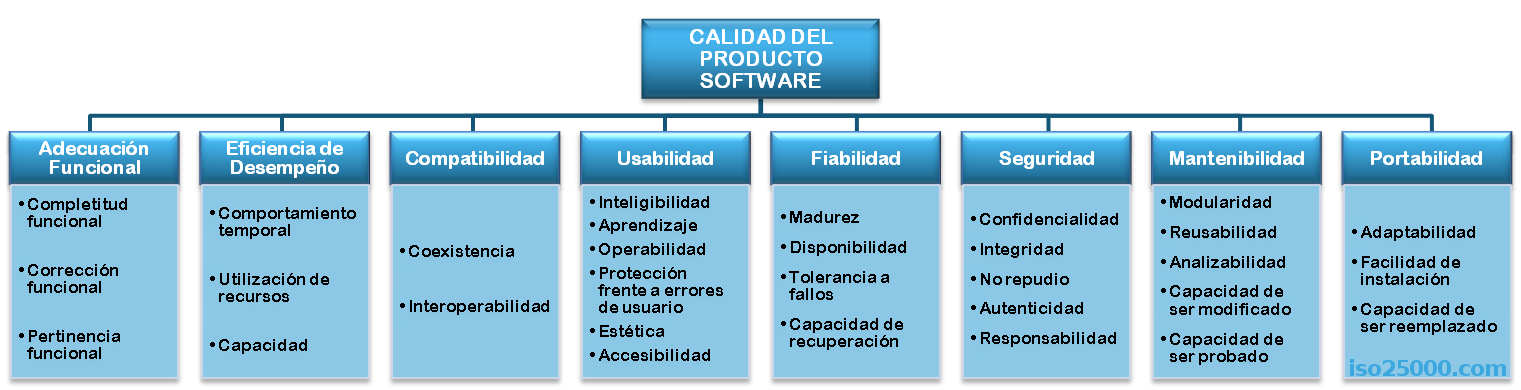
\includegraphics[width=\textwidth]{aux/nofun}
  \caption{Requisitos No funcionales}
  \label{figCasosUso}
\end{center}
\end{figure}

\begin{itemize}
	\item Seguridad
	\item Autenticación
	\item Autorización
		\begin{itemize}
			\item Definición de Roles
		\end{itemize}
	\item Disponibilidad
	\item Usabilidad
	\item Modificabilidad
	\item Testeabilidad
\end{itemize}